\chapter{Introduction}


\section{Problem}

State that it's not in my assignment to evaluate recommendation techniques, but that I use a backend system for that part. My task is the client part in figure \ref{tech_news_app_architectural_view}

\begin{figure}[!htbp]
\centering
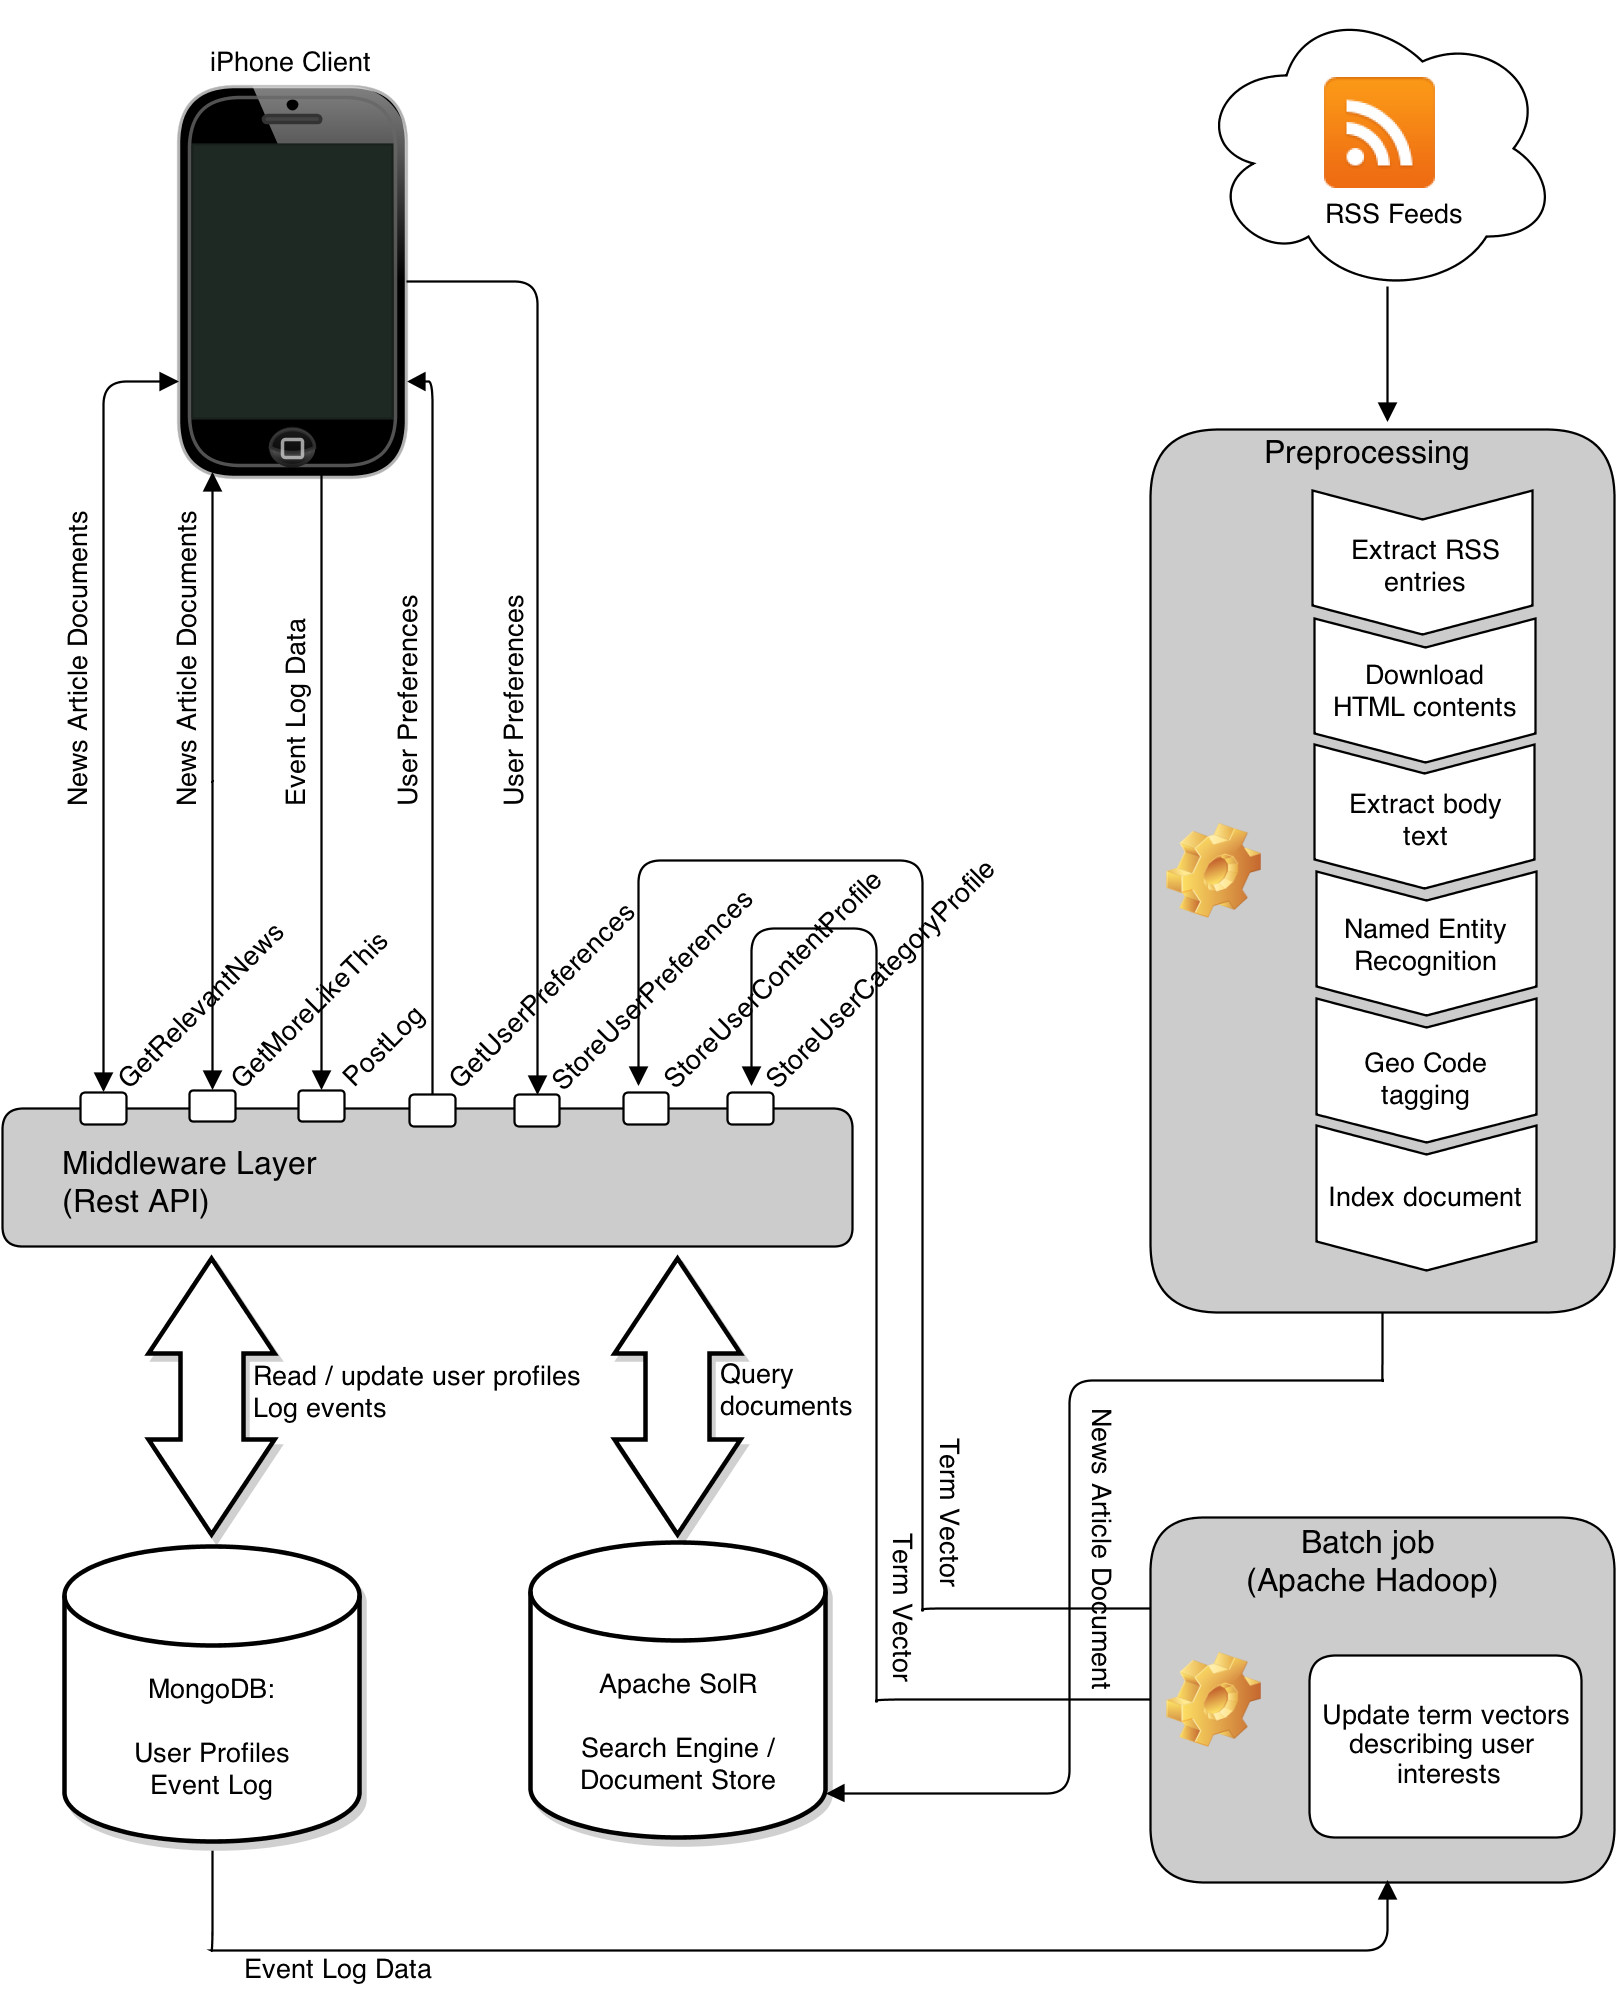
\includegraphics[width=130mm]{GFX/tech/newsAppArchitecture.png}
\caption{Conceptual drawing showing the architectural view of the whole news recommender system.}
\label{tech_news_app_architectural_view}
\end{figure}

Explain briefly how my problem evolves around an intersection of a mobile application, news application and a recommender system.

\subsection{Research questions}

GIVE A PERSONAL INTERPRETATION ON THE RESEARCH QUESTIONS

- What are possible perspectives on news in a personalized news recommender system and how are they related? (logical structure of news: articles, maps, entities, categories,...)  ... should come up with a model to show how different aspects of news are related.

(Create some figure to show how they are related, like a pin on a map with title corresponds to the name of the place in the title for instance. Or an entity like Madrugada in an entity view, can correspond to a word (Madrugada) in a text about Sivert Høyem)
\\\\
- What are particular features of mobile user interfaces that affect the mobile news user experience? (platform stuff)

(Touch gestures plays a significant role when designing a mobile app, save space wherever you can -> gestures instead of buttons, make more screens with less info instead of cluttering the screen. Only one domain per screen, type of. E.g. in this case separate map and article view.

Unable to hover with the mouse
)
\\\\
- What are relevant perspectives on news in current mobile news apps? (what do they address, and how do they implement it)

(Most apps combine categories and entities. Often the user can choose from different high level ordered categories like technology or economics, but can search for other categories and entities as well, and add these with the same hierarchical significance as the other news categories. Topics/entities can be flowers, BMW, Chelsea, cycling, etc.. Anything the user finds interesting.)
\\\\
- How can these perspective be supported on a mobile platform to increase user experience and provide maximum flexibility? (gestures vs. input, flow between related perspectives like article \& map location, etc.)  .... here we should show how we translate the model above into particular user interface features.
\\\\
-  User case: Our news recommender system

\section{Research Approach}
overall research approach

\subsection{Introduction}

- short text describing the different research strategies
\\\\

\subsection{Methodology}

- What kind of methodology will I be using (Design-science ?)

\subsection{Overall Research Phases}

- Describe the different phases in my research
\\\\
- Typisk: check out similar projects/articles -> relate to my project -> implement an demo application -> evaluate the whole shabang!

\section{Results}


\section{Report Structure}

\subsubsection{Chapter 2: Lorem}

\subsubsection{Chapter 3: Lorem}